%! Author = oli
%! Date = 12/24/23

% Preamble
%\documentclass[10pt,twocolumn,letterpaper]{article}
\documentclass[10pt]{article}
\setlength{\parindent}{0em}

\usepackage{color}

% Packages
\usepackage{amsmath}
\usepackage{chemfig}
\usepackage[utf8]{inputenc}
\usepackage{acronym}
\usepackage{hyperref}
\usepackage{subfig}
\usepackage{graphicx}
\usepackage{float}
\usepackage{tikz}
\usepackage{subcaption}
\usepackage{amssymb}
\usepackage{eurosym}
\usepackage[ngerman]{babel}
\usepackage{titlesec}
\usepackage{parskip}

\title{Filamente und mehr}
\author{Oliver Schütz}




\begin{document}

    \maketitle
    \tableofcontents

    \newpage
    \begin{abstract}
\textit{Der 3D-Druck ist ein Herstellungsverfahren, das es erlaubt, aus verschiedensten Materialien jegliche Formen herzustellen.
Mit herkömmlichen Verfahren ist dies nicht möglich.
Jedoch braucht es dafür spezielle Materialien, die entsprechende Eigenschaften aufweisen.
Hier beschränken wir uns auf Materialien, die mit dem FDM-Verfahren verarbeitet werden können, genauer gesagt auf Filamente.
FDM steht für Fused Deposition Modeling, was auf Deutsch etwa Schmelzschichtung bedeutet und ist das am weitesten verbreitete 3D-Druckverfahren.
Dabei wird ein Kunststoffdraht, das sogenannte Filament, durch eine Düse gepresst und auf einer Druckplatte Schicht für Schicht aufgetragen, woraus das Druckobjekt entsteht.
}
    \end{abstract}

    \section{Filamentherstellung}
    Es gibt verschiedene Arten von Materialien, die sich in Farbe, Form und Material unterscheiden.

    \subsection{Farben und Formen}
    Bei dem FDM-Druck kann grundsätzlich mit allen Farben und Formen gedruckt werden.
    Die verbreitetste Art ist das Filament.
    Zu Beginn der Produktion liegt das Material roh und farblos vor, z.B. als Granulat oder Pellets.
    Obwohl es üblich ist die Pellets zu Filamenten zu verarbeiten, ist es auch möglich, direkt mit den Pellets zu drucken (Pellet-Extruder).


    \begin{figure}[H]
        \centering
        \subfloat[\centering PLA]{{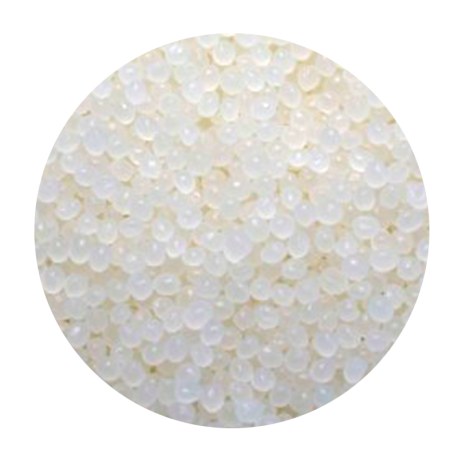
\includegraphics[width=5cm]{img/PLA-Pellets}}}%
        \qquad
        \subfloat[\centering PETG]{{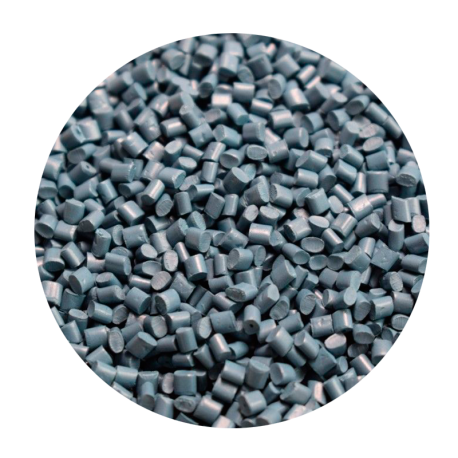
\includegraphics[width=5cm]{img/PETG-Pellets}}}%
        \caption*{Beispiel für Pellets oder Granulat als Ausgangsmaterial für Filamente}
    \end{figure}

    \subsection{Produktion}
    Im ersten Schritt vermischt man die Pellets mit Farbstoffen oder anderen Materialien, um die gewünschte Farbe zu erhalten oder die Eigenschaften des Materials zu verändern.
    Beispiele für das Beimischen von anderen Materialien sind Kohlefasern, um das Filament stabiler zu machen, TPU um es flexibler zu machen oder Holzfasern, um es wie Holz aussehen zu lassen.
    Bei teureren Filamenten wird das Gemisch anschließend noch getrocknet, um die Feuchtigkeit zu entfernen.
    Macht man dies nicht, kann es zu Blasenbildung im Filament kommen, was zu schlechteren Druckergebnissen führt.

    \begin{figure}[H]
        \centering
        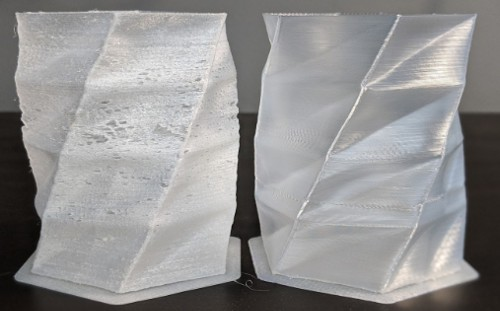
\includegraphics[width=10cm]{img/wet_filament}
        \caption*{Links: Filament mit Feuchtigkeit; Rechts: Getrocknetes Filament}
    \end{figure}

    Anschließend wird das Gemisch in einem Extruder zu Filament verarbeitet.
    Durch einen Trichter gelangt das Granulat / Pellets in eine Extrusionseinheit.
    Dort wird es durch eine Schnecke gefördert und durch gleichzeitiges Erhitzen in einen zähen Kunststoffzustand überführt.
    Am Ende der Schnecke wird das Material durch eine Düse gepresst, die den Durchmesser des Filaments bestimmt und es in die gewünschte Form bringt.

    \begin{figure}[H]
        \centering
        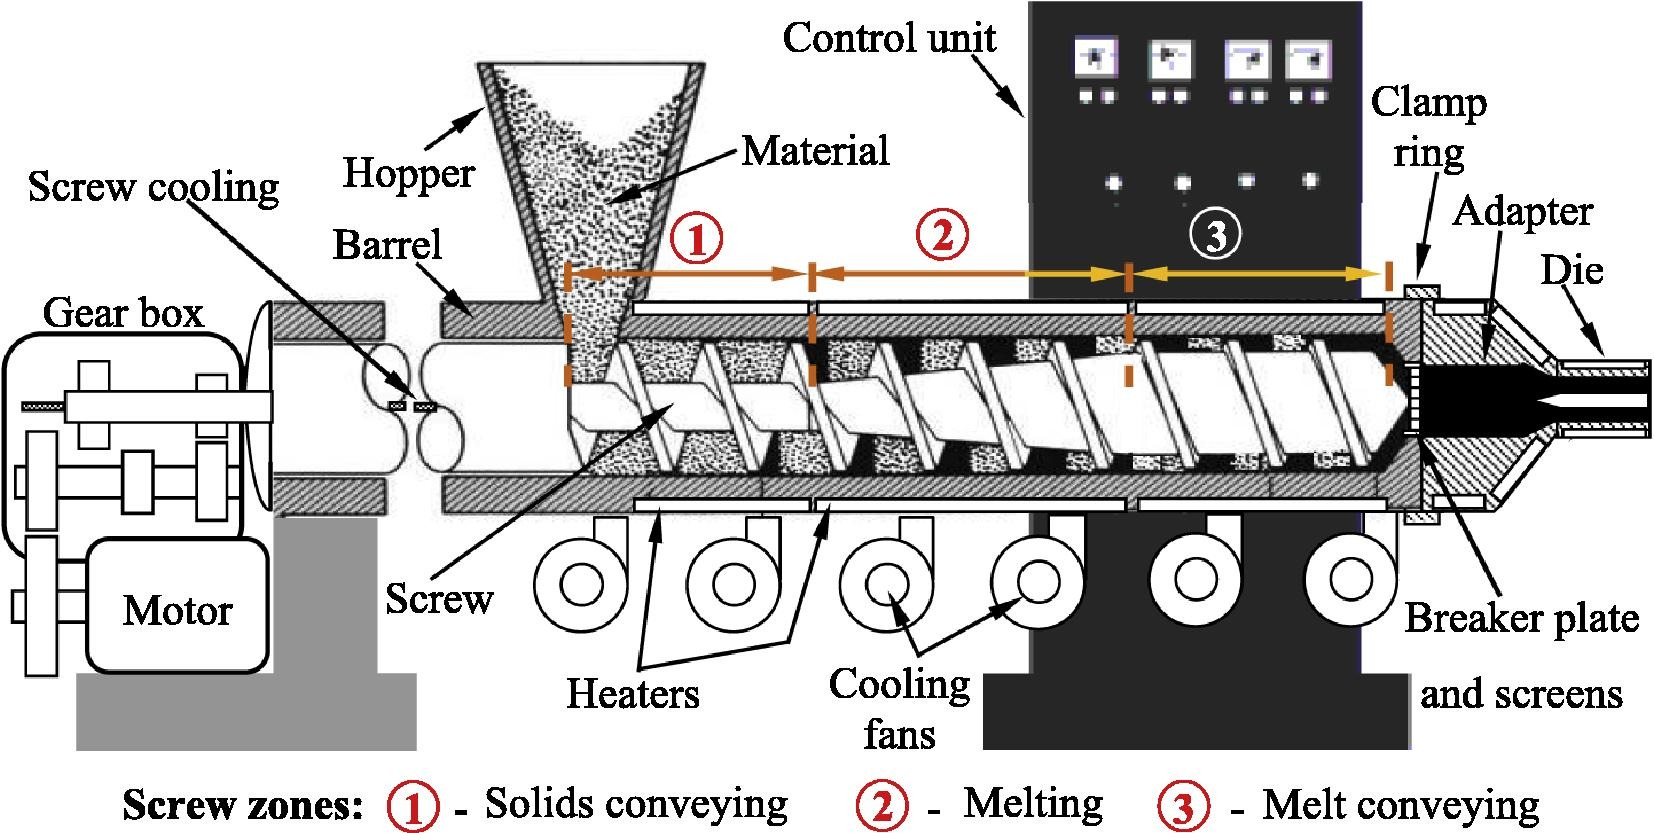
\includegraphics[width=10cm]{img/Production}
        \caption*{Extruder}
    \end{figure}

    Da das Filament nach dem Extrudieren noch heiß und sehr weich ist, würde es sich von selbst verformen.
    Deshalb wird der Filamentstrang durch eine Kühlvorrichtung geführt, das ihn stabilisiert und abkühlt.


    \begin{figure}[H]
        \centering
        \subfloat[\centering Extruder]{{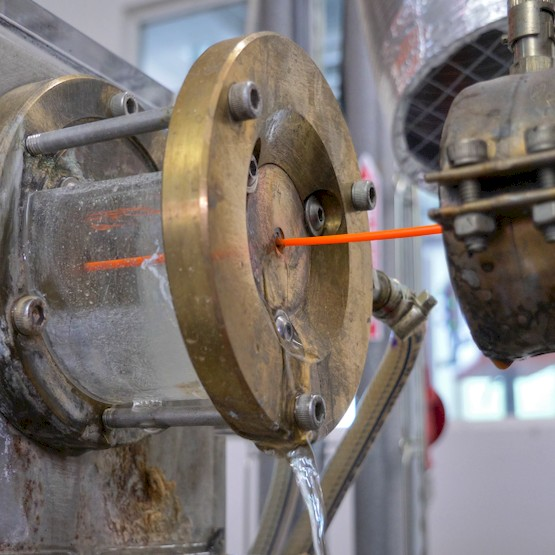
\includegraphics[width=5cm]{img/Extruder}}}%
        \qquad
        \subfloat[\centering Kühlbecken]{{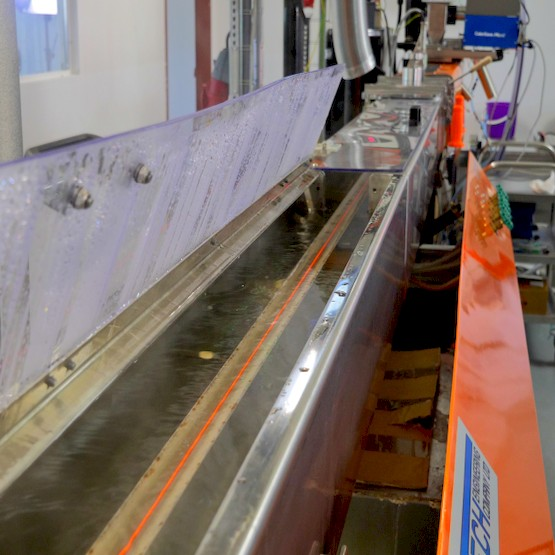
\includegraphics[width=5cm]{img/Kuehler}}}%
    \end{figure}

    \newpage
    Abschließend wird das Filament noch auf Toleranz des Durchmessers geprüft und auf die Spulen gewickelt.

    \begin{figure}[H]
        \centering
        \subfloat[\centering Toleranzmessung]{{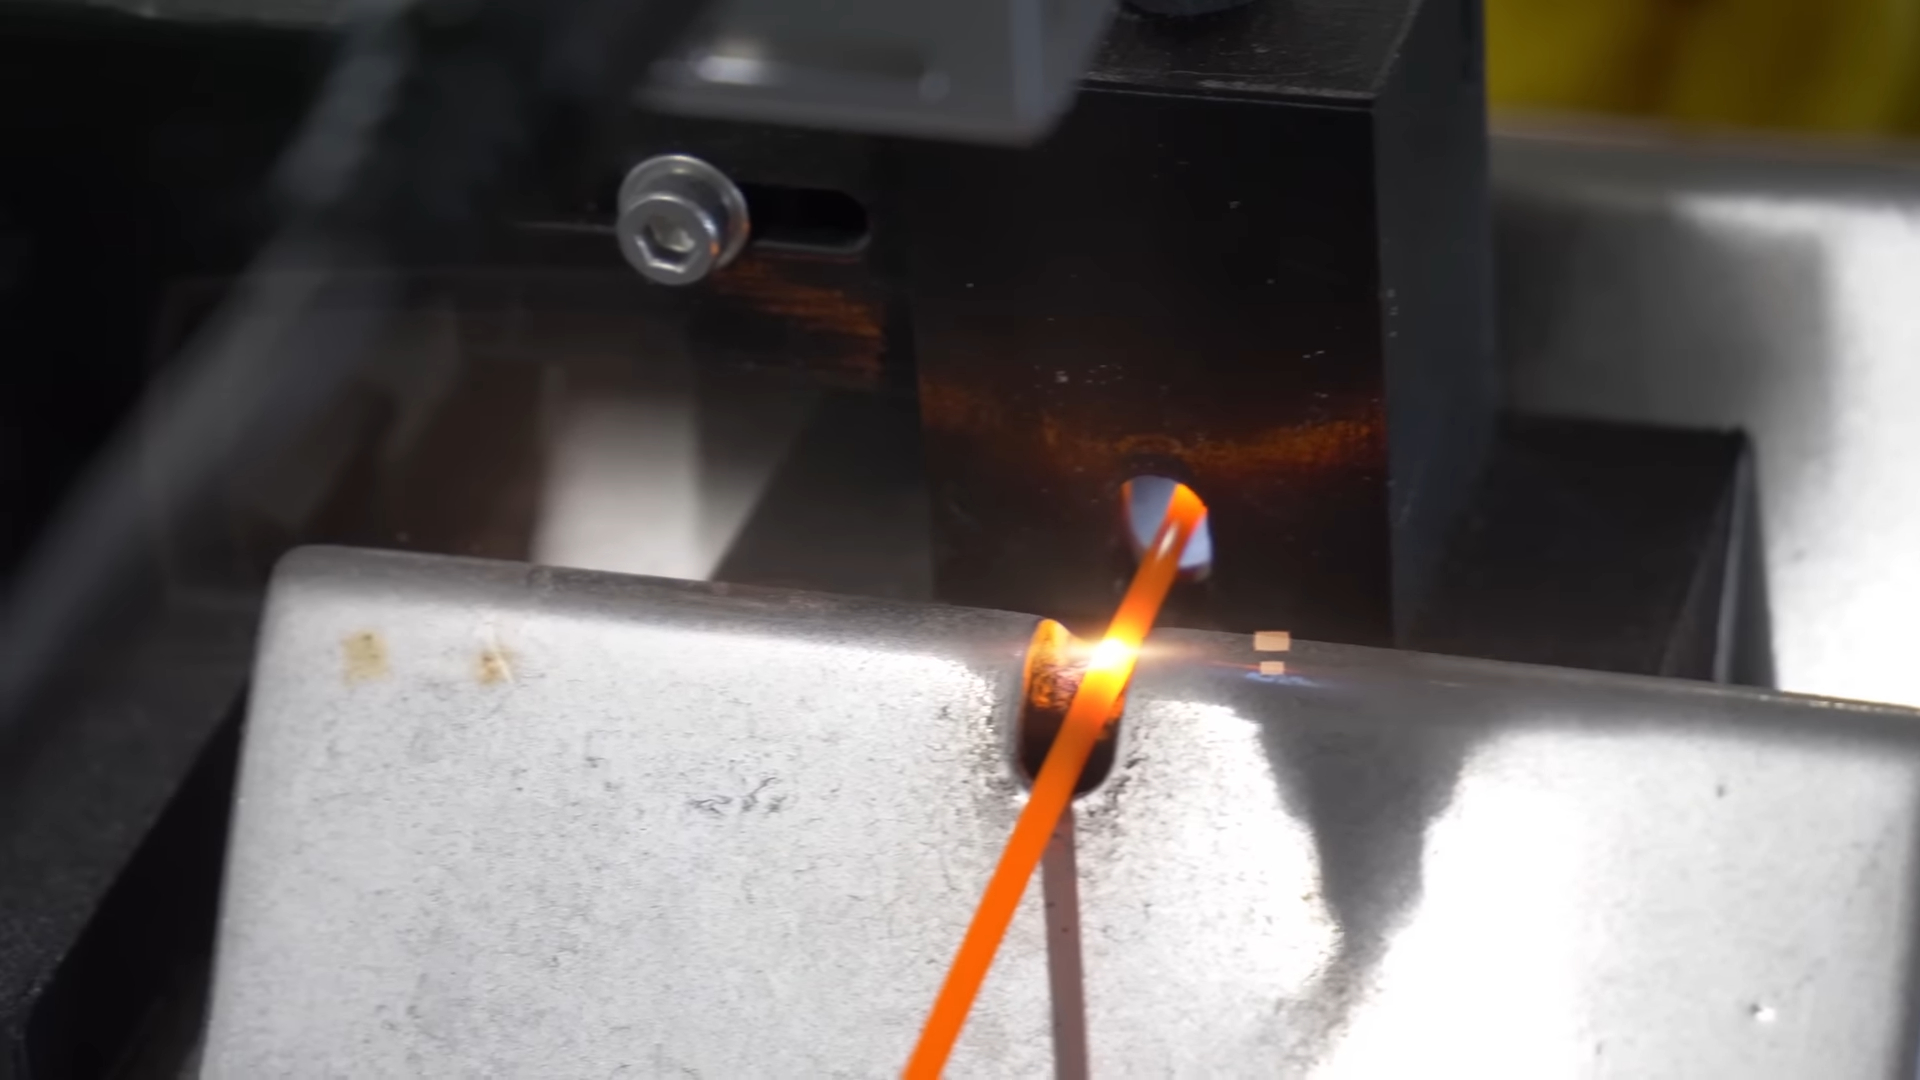
\includegraphics[width=5cm]{img/Qualität}}}%
        \qquad
        \subfloat[\centering Wickelung]{{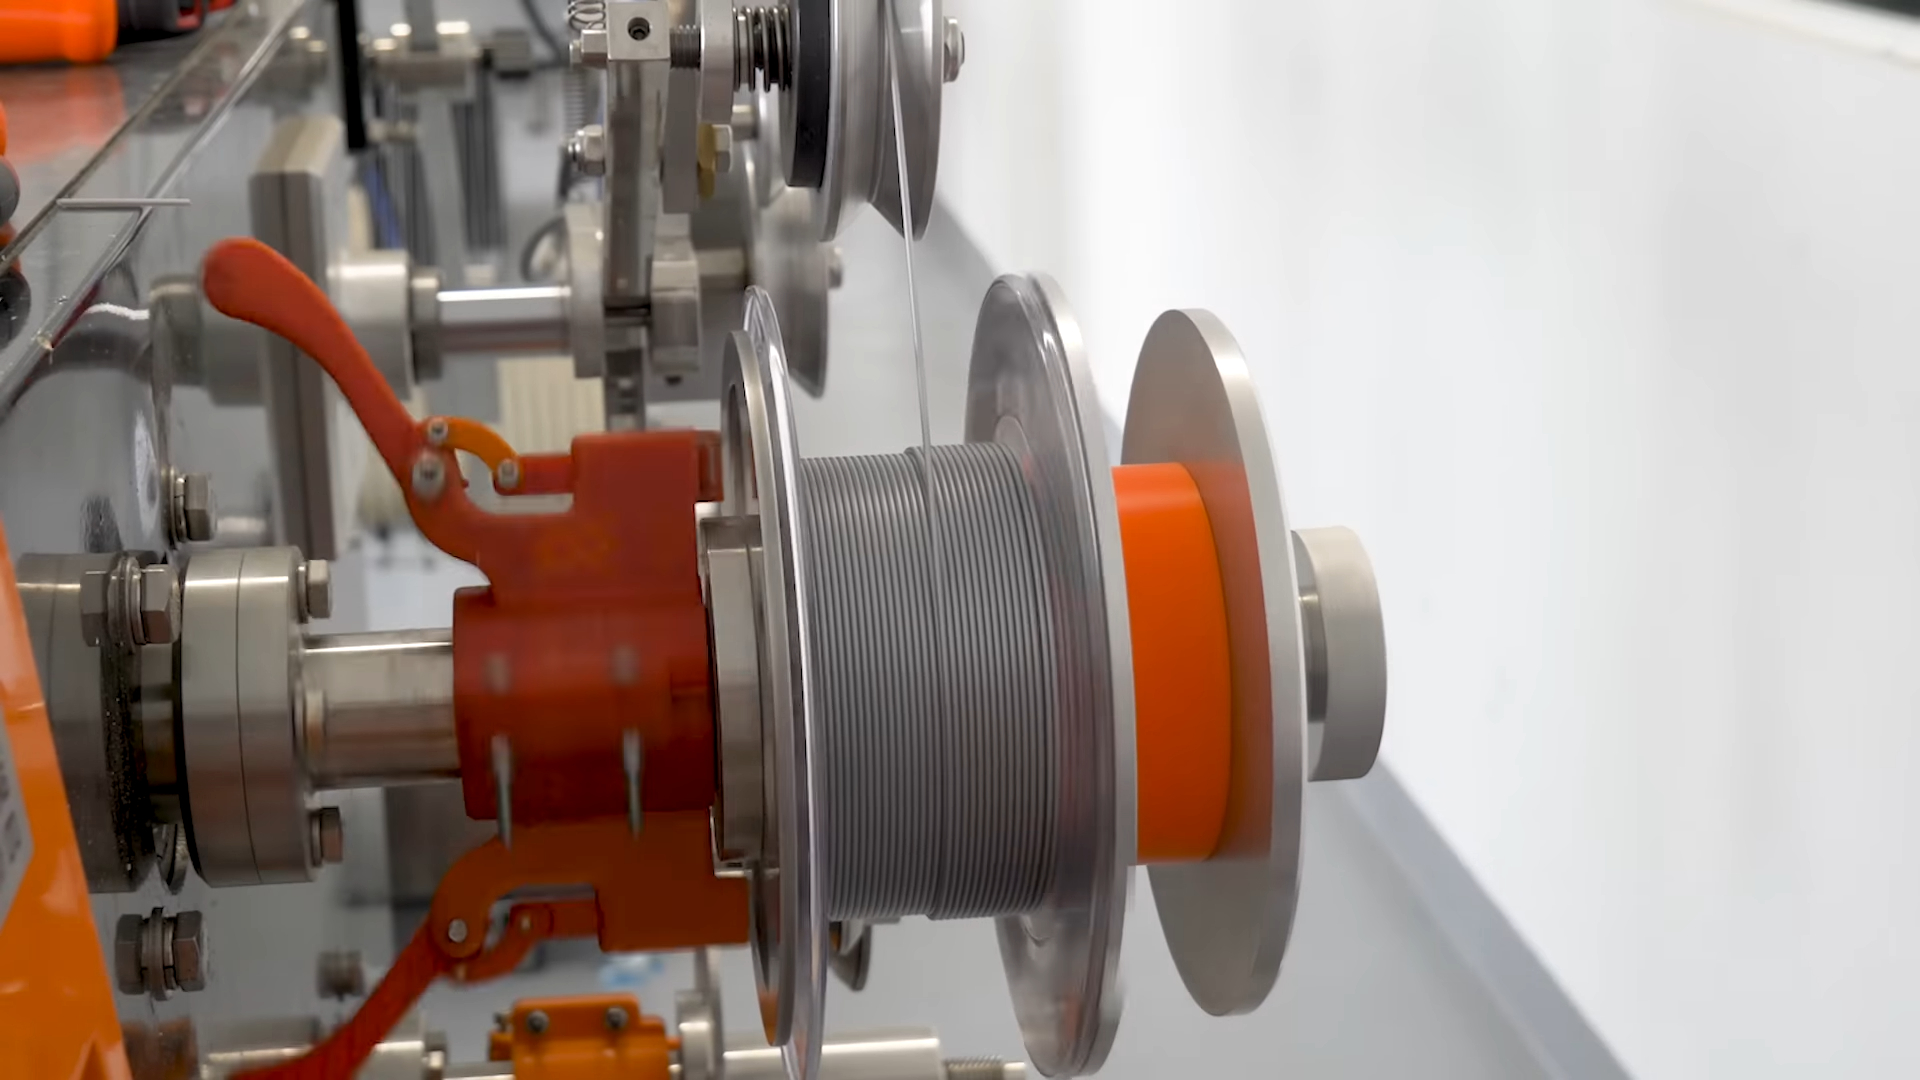
\includegraphics[width=5cm]{img/Wickellung}}}%
    \end{figure}


    \subsection{Recycling}
    Wie bei fast allen Herstellungsverfahren, entsteht auch beim 3D-Druck Abfall.
    Das Filament kann jedoch wieder eingeschmolzen und zu neuen Filamenten verarbeitet werden.
    Dazu wird das Filament geschreddert und zu Granulat verarbeitet.
    Anschließend kann es wieder als Ausgangsmaterial für die Filament Herstellung verwendet werden.
    Zudem lassen sich auch weitere Kunststoffprodukte wie PET-Flaschen oder Spritzgussteile recyceln, auch wenn das daraus hergestellte Filament nicht optimal für den 3D-Druck geeignet ist.


    \begin{figure}[H]
        \centering
        \subfloat[\centering Filament Reste]{
            \centering
            \begin{tikzpicture}
                \clip (0,0) circle (1.5cm) node {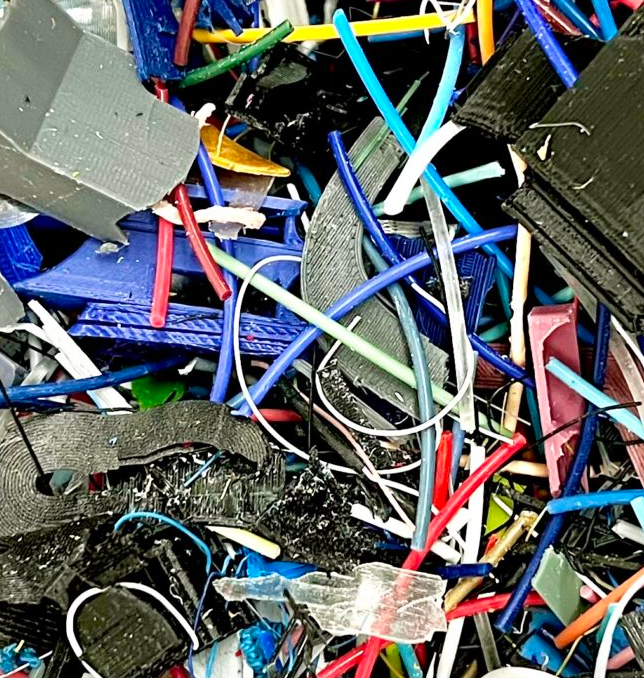
\includegraphics[width=3cm]{img/Reste}};
            \end{tikzpicture}
        }%
        \raisebox{1.5cm}{\LARGE$\longrightarrow$}%
        \subfloat[\centering Granulat]{
            \centering
            \begin{tikzpicture}
                \clip (0,0) circle (1.5cm) node {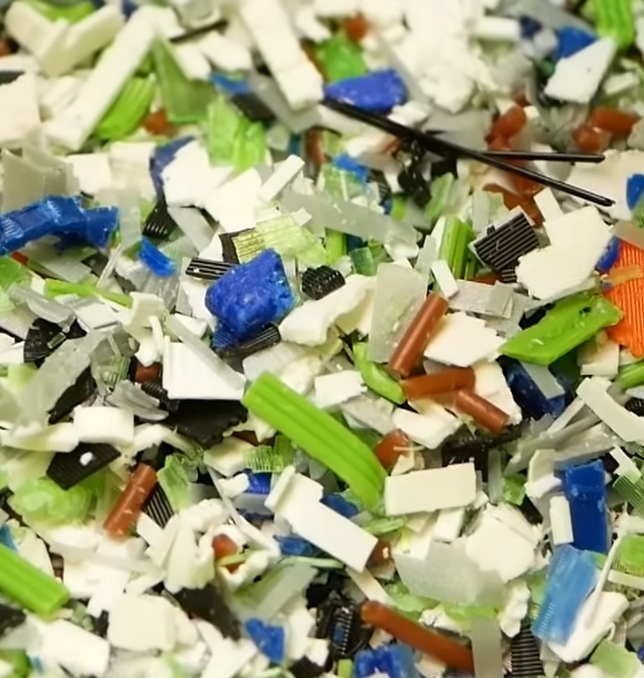
\includegraphics[width=3cm]{img/Geschreddert}};
            \end{tikzpicture}
        }%
        \raisebox{1.5cm}{\LARGE$\longrightarrow$}%
        \subfloat[\centering Filament]{
            \centering
            \begin{tikzpicture}
                \clip (0,0) circle (1.5cm) node {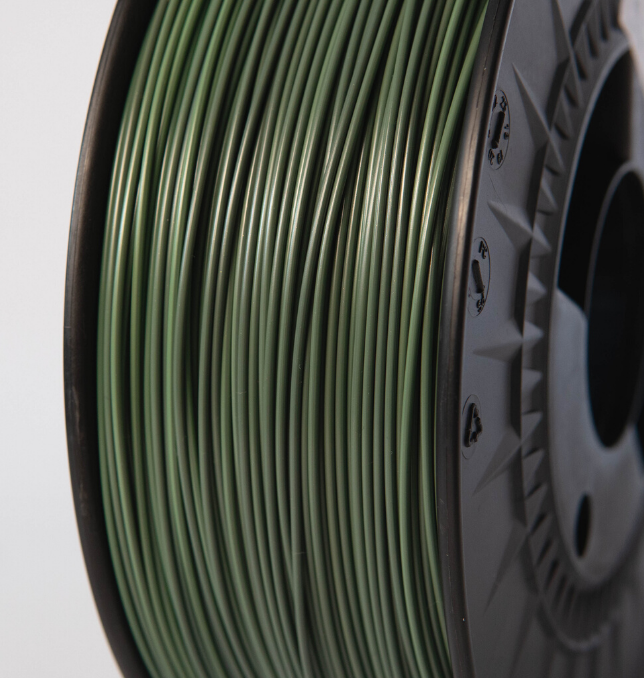
\includegraphics[width=3cm]{img/Filament}};
            \end{tikzpicture}
        }%
    \end{figure}


    \newpage
    \section{Kunststoffe und ihre Eigenschaften}
    Wie bereits erwähnt, kann man so gut wie alle Kunststoffe zum 3D-Druck verwenden.
    Damit ein Kunststoff jedoch für den FDM-Druck geeignet ist, müssen bestimmte Dinge beachtet werden.

    \begin{itemize}
        \item Schmelztemperatur
        \item Wärmeformbeständigkeit
        \item Schmelzviskosität
        \item Schrumpfverhalten
        \item Abrasivität
    \end{itemize}
    Die Schmelztemperatur darf nicht zu hoch sein, da der Kunststoff sonst zu langsam abkühlt und sich dadurch verzieht.
    Sie darf aber auch nicht zu niedrig sein, da der Kunststoff bei Wärme nicht formbeständig genug ist und sich dadurch auch ungewollt verformt.
    Ungewolltes Verformen aufgrund von Wärme ist das sogenannte Warping. \\
    Ist die Viskosität des Kunststoffs zu hoch, kann er nicht mehr durch die Düse gepresst werden und verstopft diese. \\
    Ist die Viskosität zu niedrig, kann der Kunststoff nicht mehr in Form gehalten werden und verläuft. \\
    Wenn der Kunststoff nach dem Abkühlen zu sehr schrumpft, kann sich das Druckobjekt vom Druckbett lösen und die Genauigkeit der Druckergebnisse ist nicht mehr gewährleistet. \\
    Ist der Kunststoff oder ein Zusatzmaterial im Filament abrasiv, dann reibt es die Düse ab und beschädigt diese. \\
    Um abrasives Material zu drucken, gibt es spezielle Düsen, die z.B. aus gehärtetem Stahl bestehen oder einen Edelstein an der Spitze haben. \\

    \begin{figure}[H]
        \centering
        \subfloat[\centering Stahl Düse]{{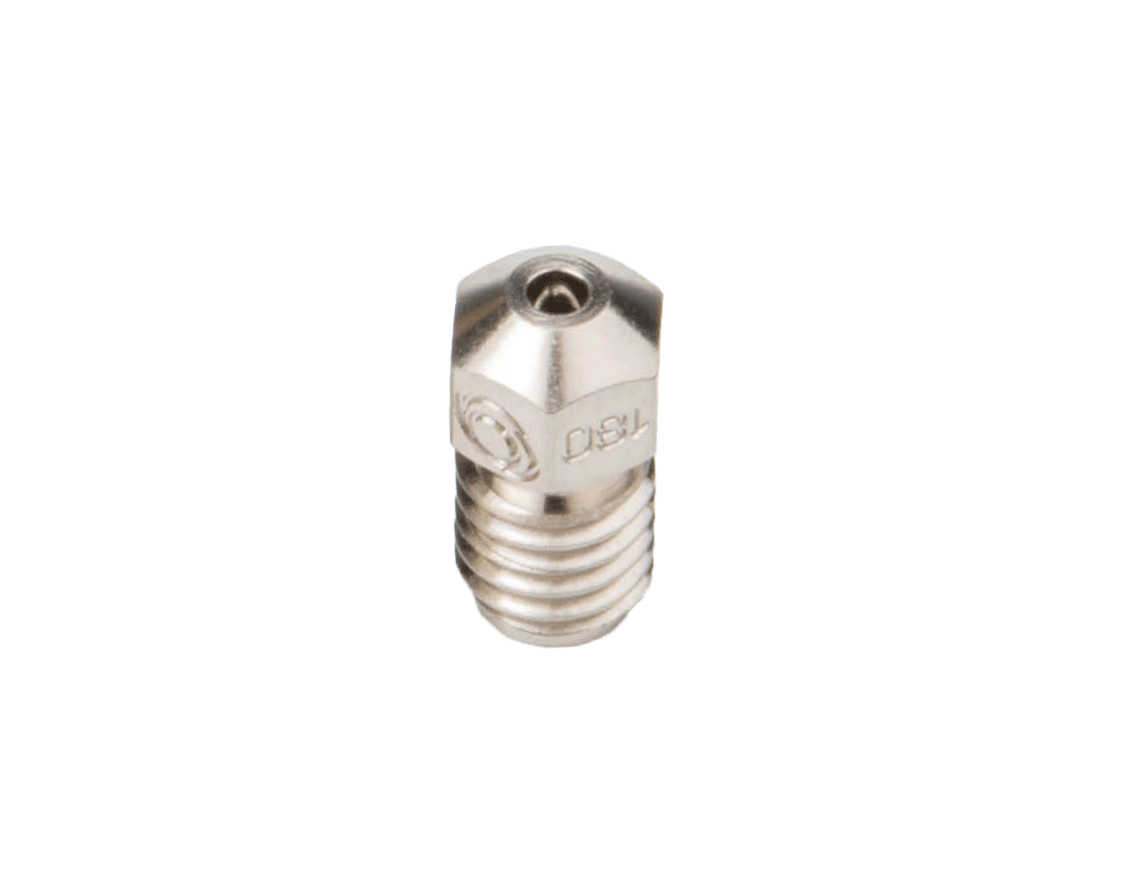
\includegraphics[width=4cm]{img/Steel_Nozzle}}}%
        \qquad
        \subfloat[\centering Rubin Spitze]{{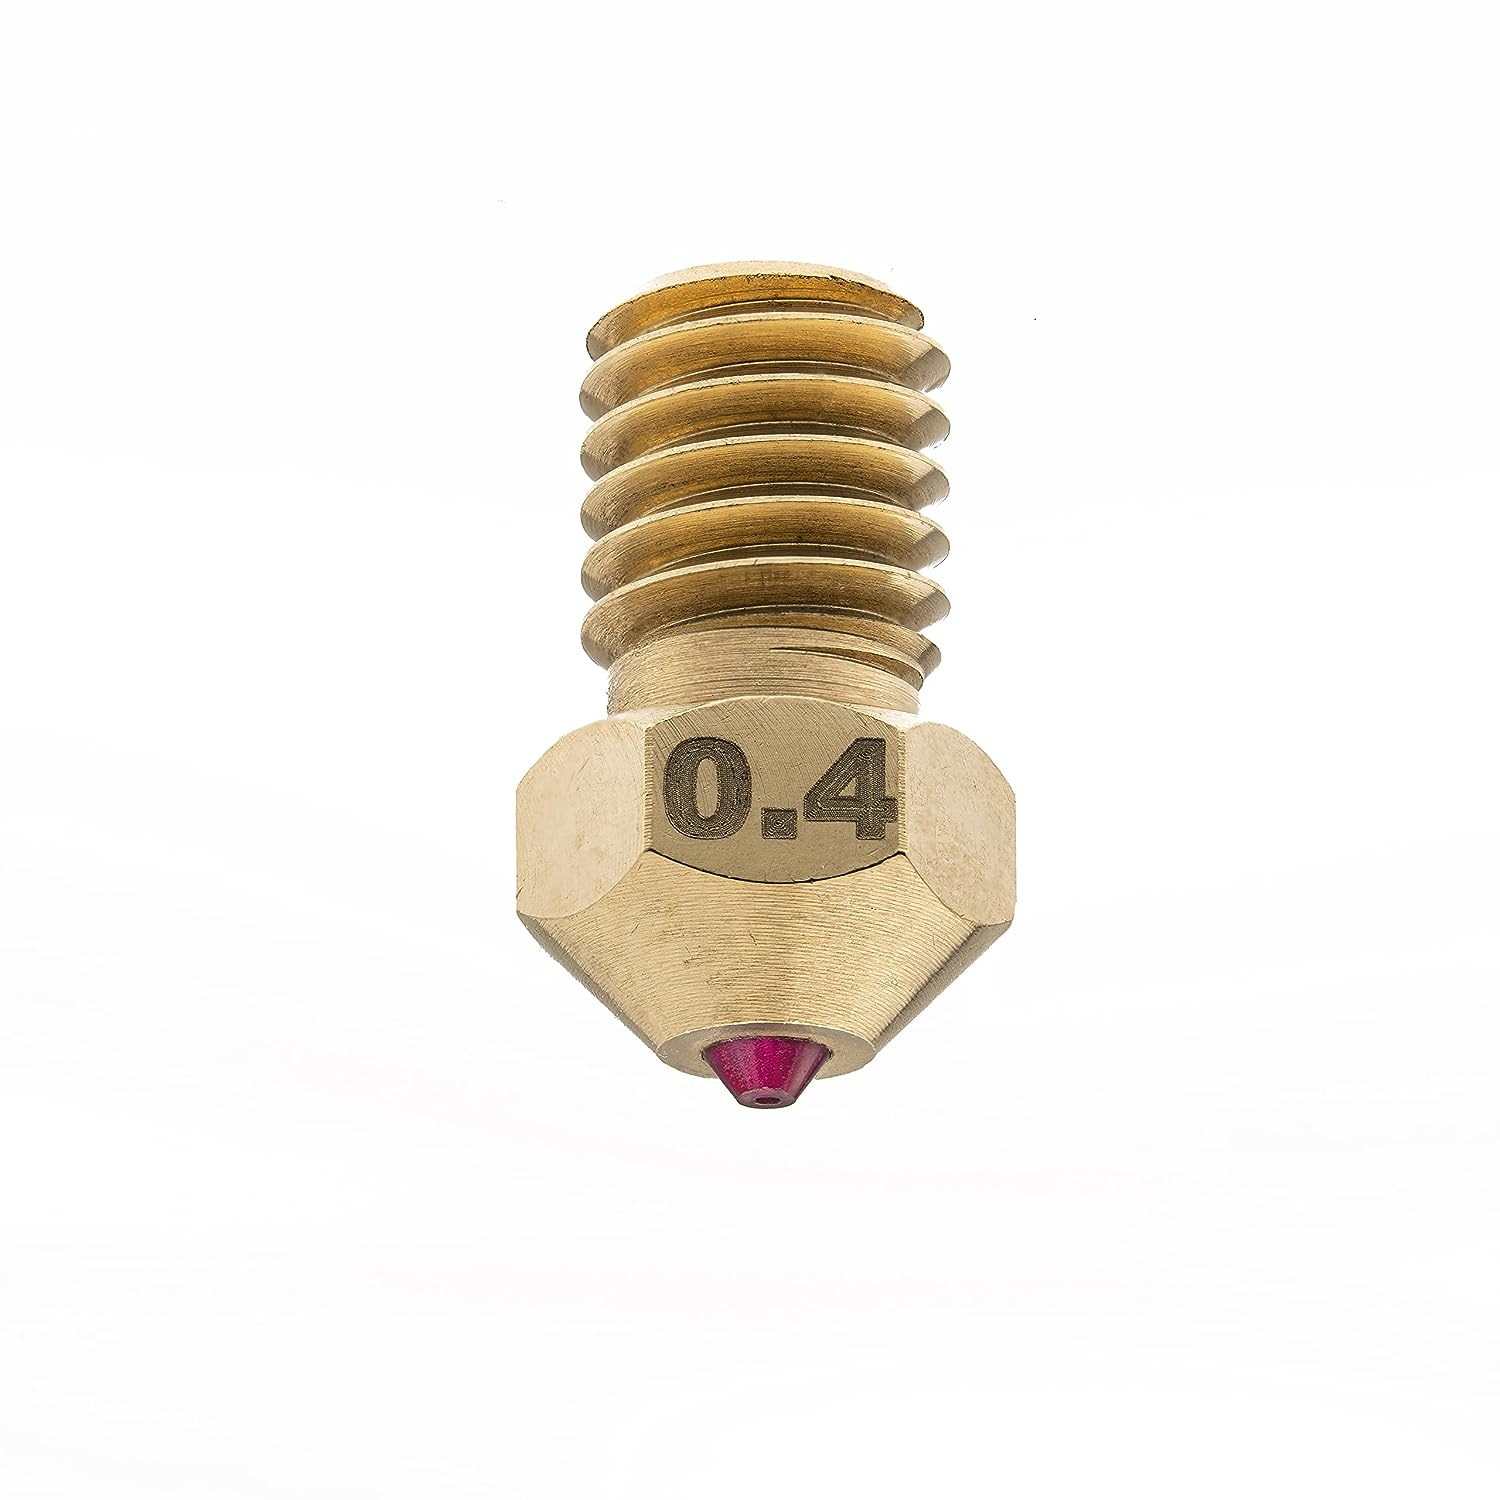
\includegraphics[width=4cm]{img/Ruby_nozzle}}}%
    \end{figure}

    \newpage
    \subsection{Filamente}
    Zu den gängigsten Filamentarten gehören PLA, PETG, ABS / ASA, TPU, Nylon und PC.
    PLA ist das am weitesten verbreitete Filament, das aus Mais hergestellt wird und biologisch abbaubar ist.
    Es ist einfach zu drucken, da es eine geringe Schmelztemperatur hat und kann daher sehr schnell gedruckt werden, es ist auch nicht abrasiv und muss auch nicht in einem beheizten Druckraum gedruckt werden.
    Es ist jedoch nicht sehr stabil, recht spröde und wird bereits bei 60°C weich.
    Zudem ist es absolut nicht chemisch beständig und zersetzt sich bei UV-Strahlung.
    Daher eignet es sich für Dekorationen, oder für Prototypen, die nicht lange halten müssen oder für Teile, die nicht mechanisch belastet werden.
    Etwas beständiger ist PETG. Es ist etwas flexibler als PLA und hat eine höhere Schmelztemperatur.
    PETG ist zudem stabiler und chemisch beständiger als PLA, jedoch nicht UV-beständig.
    Es eignet sich für mechanische Teile mit geringer Belastung oder Möbel im Innenbereich.
    ABS ist noch stabiler und steifer als PETG, es kann auch höheren Temperaturen standhalten, jedoch muss es in einem beheizten Druckraum gedruckt werden, da es sonst zu Warping kommt.
    Abgesehen vom 3D-Druck wird es im Spritzguss oft verwendet z.B. Legosteine, Playmobil oder auch Auto- und Motorradteile.
    ABS hat den Nachteil oder auch Vorteil, dass es durch Aceton aufgelöst werden kann, was man sich beim 3D-Druck zunutze machen kann, um Teile zu verkleben oder zu glätten.
    ASA ist eine Variante von ABS, die UV-beständig ist und sich daher für den Außenbereich eignet.
    TPU ist ein flexibles Filament, das sich für Dichtungen, Stoßdämpfer oder Schutzhüllen eignet.
    TPU ist daher aber schwerer zu drucken, da das Zahnrad des Extruders das Filament schlechter greifen kann.

    Nylon und Polycarbonat sind sehr stabile Filamente, die sich für mechanische Teile eignen, die hohen Belastungen ausgesetzt sind.
    Sie sind aber sehr schwer zu drucken, da sie eine hohe Schmelztemperatur haben und sehr abrasiv sind.

    Es gibt natürlich noch viele weitere Filamente, z.B. Holzfilament für Holzoptik oder PVA für Stützstrukturen, die sich in Wasser auflösen, aber sie sind nicht so weit verbreitet. \\

    \begin{table}[H]
        \begin{tabular}{|l|c|c|c|c|c|c|}
            \hline
            \textbf{Filament} & \textbf{PLA} & \textbf{PETG} & \textbf{ASA} & \textbf{TPU} & \textbf{Nylon} & \textbf{PC} \\
            \hline
            \textbf{Drucktemperatur} & 190-230°C & 230-260°C & 225-255°C & 210-230°C & 220-270°C & 260-310°C \\
            \hline
            \textbf{Druckbett} & 60°C & 80°C & 90-110°C & 60°C & 70-90°C & 80-120°C \\
            \hline
            \textbf{Preis pro kg} & 20-30\officialeuro & 20-30\officialeuro & 20-30\officialeuro & 20-30\officialeuro & 40-60€ & 40-60\officialeuro \\
            \hline
            \textbf{Stabilität} & Niedrig & Mittel & Hoch & Mittel & Hoch & Hoch \\
            \hline
            \textbf{Steifheit} & Hoch & Mittel & Hoch & Niedrig & Mittel & Hoch \\
            \hline
            \textbf{UV-Beständigkeit} & Nein & Nein & Ja & Nein & Nein & Ja \\
            \hline
            \textbf{Chemische Beständigkeit} & Niedrig & Mittel & Mittel & Mittel & Mittel & Hoch \\
            \hline
        \end{tabular}
    \end{table}

    \newpage

    \section{PLA}
    PLA bzw. Polymilchsäure ist ein Biopolymer, das aus erneuerbaren Ressourcen wie Weizen, Stroh, Mais und Hirse gewonnen wird.
    Es ist umweltfreundlich, da es von Mikroben zu Wasser und Kohlendioxid abgebaut werden kann.
    Zudem liegt die Verarbeitungstemperatur zwischen 170 und 230°C, wodurch es für Extrusions-, Spinn-, biaxiale Streck- und Spritzblasformverfahren geeignet ist.
    PLA hat auch eine gute Biokompatibilität, Bioabbaubarkeit, Glanz und Transparenz sowie antibakterielle, flammhemmende, öl- und wasserabweisende Eigenschaften.
    Dadurch kann es in vielen Bereichen eingesetzt werden, z.B. als Verpackungsmaterialien, Vliesstoffe, Kleidung und medizinische Anwendungen (Fäden, Implantate, OP-Material).

    \subsection{Milchsäure}
    Milchsäure wurde erstmals aus fermentierter Milch extrahiert, und ist ein wichtiger Bestandteil des glycolytischen Energiekreislaufs von Organismen.
    Das Molekül der Milchsäure enthält ein asymmetrisches Kohlenstoffatom auch chirales Zentrum genannt, das optisch aktiv ist.
    Ist ein Molekül optisch aktiv, bedeutet das, dass es zwei optische Isomere gibt, die sich zueinander verhalten wie Bild und Spiegelbild.
    Das bedeutet, es gibt zwei optische Isomere, L-Milchsäure und D-Milchsäure.
    Einfach gesagt, dreht L-Milchsäure polarisiertes Licht nach links und D-Milchsäure nach rechts.
    D-Milchsäure wird aus Tiermuskeln gewonnen, während L-Milchsäure durch Fermentation gewonnen wird.

    \begin{figure}[H]
        \centering
        \subfloat[\centering L-lactic acid]{\chemfig{[:-30]HO-(<[:210]H)(<:[:-40]CH_{3})-[:30](=[2]O)(-[:-30]OH)}}%
        \qquad
        \subfloat[\centering D-lactic acid]{\chemfig{[:-30]HO-(<[:210]H_{3}C)(<:[:-40]H)-[:30](=[2]O)(-[:-30]OH)}}%
    \end{figure}

    Die Fermentation wird durch Bakterien durchgeführt, die Zucker in Milchsäure umwandeln, welcher von Mais oder Kartoffeln gewonnen wird.
    Dies umfasst die Fermentation von Stärke, Glukose, Laktose und Maltose.
    Der Ablauf der Fermentation dauert in der Regel 3-5 Tage und wird bei niedrigem pH-Wert (5.0), niedrigem Sauerstoffgehalt und einer Temperatur von etwa 40°C durchgeführt.
    Jedoch wird die Milchsäure mit der Zeit giftig, da sich die Konzentration der Milchsäure erhöht.
    Um die Toxizität zu reduzieren, wird Ammoniak oder Natriumhydroxid hinzugefügt, um die Milchsäure zu neutralisieren.
    Etwas neuere Methoden zur Herstellung von Milchsäure umfassen die Ultrafiltration, Färbung und Elektrodialyse.
    Auch wenn diese Verfahren von der FDA zugelassen wurden, sind die Ausgangsstoffe im Allgemeinen giftig.

    \subsection{Polymilchsäure}

    Will man nun aus der Milchsäure das PLA herstellen so muss diese polymerisiert werden, man erhält dann die Polymilchsäure.
    Wie bereits erwähnt, ist Milchsäure ein chirales Molekül mit zwei optischen Isomeren, L- und D-Milchsäure.
    Aus diesen beiden Isomeren können drei Formen von Polymilchsäure synthetisiert werden: Poly-L-Milchsäure (PLLA), Poly-D-Milchsäure (PDLA) und Poly-D,L-Milchsäure (PDLLA).
    Das erste synthetisierte PLA war PLLA, das aus L-Milchsäure hergestellt wurde.
    Es wurde jedoch festgestellt, dass PLLA aufgrund seiner hohen Kristallinität und langsamen Abbaurate eine Entzündungsreaktion im Körper auslösen kann.
    Die zweite Form PDLA dagegen, wird schneller abgebaut.
    Verwendet man nun die dritte Form PDLLA, so kann man diese Probleme vermeiden und dennoch die Vorteile von PLLA nutzen.
    Z.B. ist PLLA stabiler als PDLA. \\ \\
    Nun gibt es drei Methoden, PLA mit einem Molekulargewicht größer als 10.000 g/mol herzustellen:
    \begin{enumerate}
        \item Direkte Kondensationspolymerisation
        \item Azeotrope Dehydratisierungskondensation
        \item Lactid-Ringöffnungspolymerisation
    \end{enumerate}

    \begin{figure}[H]
        \centering
        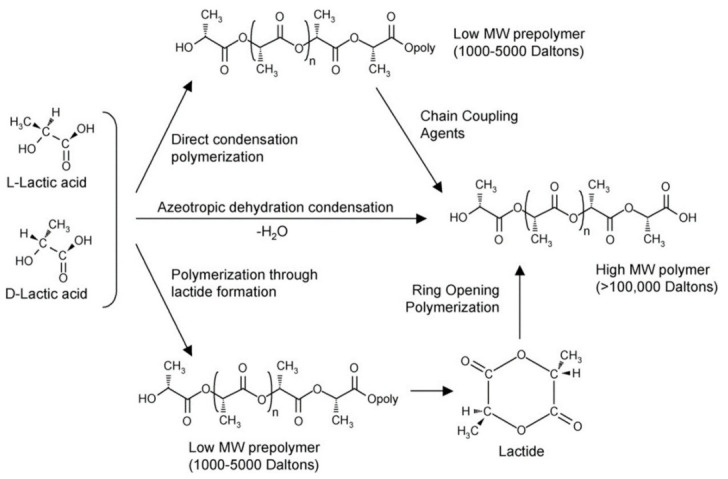
\includegraphics[width=10cm]{img/PLA_synthese}
        \caption*{Polymerisation von Milchsäure zu Polymilchsäure}
    \end{figure}

    \subsection{Kondensationspolymerisation}
    Durch die Kondensationspolymerisation kann leicht und günstig niedermolekulares PLA hergestellt werden.
    Dies geschieht durch die Kondensation von Hydroxyl- und Carboxylgruppen in äquimolaren Konzentrationen.
    Im zweiten Schritt werden Kupplungsmittel und Veresterungsadjuvantien hinzugefügt, die die PLA modifizieren und die Kette verstärken.
    Dieser Schritt ist deutlich kostenintensiver, als der Erste.
    Im nachfolgenden Produktionsprozess war es möglich die Polymerisation durch eine effizientere Wasserentfernung zu beschleunigen.
    Zinnverbindungen haben sich als effektive Katalysatoren erwiesen, jedoch müssen diese nach der Polymerisation entfernt werden, da sie giftig sind.
    Dieser Katalysator kann dafür nicht im medizinischen Bereich eingesetzt werden.

    \subsection{Ringöffnungspolymerisation}
    Die Ringöffnungspolymerisation wird im industriellen Maßstab zur Herstellung von hochmolekularem PLA verwendet.
    Um eines der drei Isomere mit hohem Molekulargewicht zu erhalten, wird zunächst die Milchsäure bei 115-179°C kondensiert, das Kondenswasser und Mesomilchsäure entfernt und anschließend umkristallisiert.
    In Industrieanlagen wird zwar dieses Schema verwendet, jedoch in unterschiedlichen Reaktoren und mit unterschiedlichen Reinigungsmethoden.
    Zum Beispiel ein Verfahren mit reduziertem Druck-Rückfluss, um Restwasser, Milchsäure, Oligomere und teilweises Lactid zu entfernen.
    Andere Methoden verwenden einen Mehrstufen-Schmelzrekristallisator oder Inertgas, um Lactid zu entfernen, umzukristallisieren und zu reinigen.
    Es können auch schwach alkalische Wasser-/Lösungsmittel-Systeme und Gasphasen-Umkristallisation verwendet werden, um Lactid zu extrahieren. \\ \\

    Je nach Katalysator kann eines der folgenden drei Polymerisationsmechanismen verwendet werden:

    \begin{itemize}
        \item Kationisch
        \item Anionisch
        \item Koordinations-/Insertionsmechanismus
    \end{itemize}

    Kationische Initiatoren sind protische Säuren, Lewis-Säuren und alkylierende bzw. acylierende Reagenzien.
    Es wurde festgestellt, dass Triflsäure und Methyltriflat Lactid effektiv induzieren können.

    Anionische Initiatoren dagegen führen zu inkosistenten Polymerisationen und Racemisierung durch Deprotonierung.
    Es wird davon abgeraten, Butyllithium oder Kronenether-Initiatoren zu verwenden, da diese Metallionen enthalten, die zu Toxizitätsproblemen führen können.
    Besser geeignet sind primäre Alkoxide, 6-Valerolacton oder Polyethylenglykol.
    Beide dieser Methoden führen zu geringer Verunreinigung.
    Verwendet man Zinn (II) und Zink während der Synthese, erhälte man die reinste Polymilchsäure, z.B. Zinn (II)-di-2-ethylhexanoat.
    Zinnverbindungen, Aluminiumalkoxide, Seltenerdverbindungen laufen alle über Koordinations-/Insertionsmechanismen ab.
\end{document}







